%
% management.tex
%
% Copyright The GOLDS-UFSC Contributors.
%
% GOLDS-UFSC Documentation
%
% This work is licensed under the Creative Commons Attribution-ShareAlike 4.0
% International License. To view a copy of this license,
% visit http://creativecommons.org/licenses/by-sa/4.0/.
%

%
% \brief Mission management chapter.
%
% \author Gabriel Mariano Marcelino <gabriel.mm8@gmail.com>
%
% \version 0.3.0
%
% \date 2023/06/13
%

\chapter{Concept of Operations} \label{ch:conops}

\section{Introduction}

This chapter describes the \ac{CONOPS} for Catarina-A1, a satellite within the Catarina Constellation, providing insights into its on-orbit operations and mission timeline.

Following this, a concise overview of the mission, including its objectives and structure, is presented. Subsequently, the operational modes of the payloads (\ac{EDC} and ExpLoRa) and service module are outlined, showcasing the interactions between subsystems and between the Space and Ground Segments for a comprehensive understanding of the mission's dynamics.

\subsection{Mission description}

Catarina-A1 was specifically designed to contribute to the Catarina Constellation mission, aimed at environmental data collection applications. Its primary objective is to gather data from one \ac{DCP} located in SC for a technological demonstration for the next space systems of the Catarina Constellation. A secondary goal is to contribute as part of the \ac{SBCD}. The collected data is then redistributed through the \ac{SINDA}.

For this matter, Catarina-A1 will use the \ac{EDC}, a \ac{INPE}'s payload specifically developed for CubeSats, designed to receive data from \acp{DCP}. The satellite will also have a secondary payload, ExpLoRa, developed by SpaceLab's team. For the service module, the FloripaSat-2 platform will be used (which is heavily based on the FloripaSat-1 platform).

As previously mentioned, the primary payload is the \ac{EDC}, developed by \ac{INPE}, which enables communication between CubeSats and \acp{DCP}. On the other hand, ExpLoRa serves as a secondary experiment, showcasing the potential use of CubeSats in \ac{IoT} applications. This approach aligns with the broader trend of integrating satellite communications and the \ac{IIoT} across diverse sectors, including agriculture, energy, and transportation.

For the service module, it is based on the FloripaSat-1 platform, and its main function is to transmit the received data to the Ground Segment through the main communication link provided by the satellite.

\subsection{Operational mission objectives}

The main mission objectives outlined in \autoref{sec:mission_objectives} revolve around the reception and transmission of data from \acp{DCP}. Additionally, a secondary objective emerged following the definition of the post-SRR payload, aimed at showcasing CubeSats' utility in an \ac{IoT} application. In summary, the mission objectives can be succinctly summarized as follows:

\begin{itemize}
    \item Receive data from one \ac{DCP} station installed in Santa Catarina;
    \item Transmit the received data to the Ground Segment through the satellite's main communication link;
    \item Provide data through \ac{SINDA} to all registered users;
    \item Receive data from a SpaceLab's \ac{IoT} application.
\end{itemize}

\section{Mission structure}

\begin{figure}[!ht]
    \begin{center}
        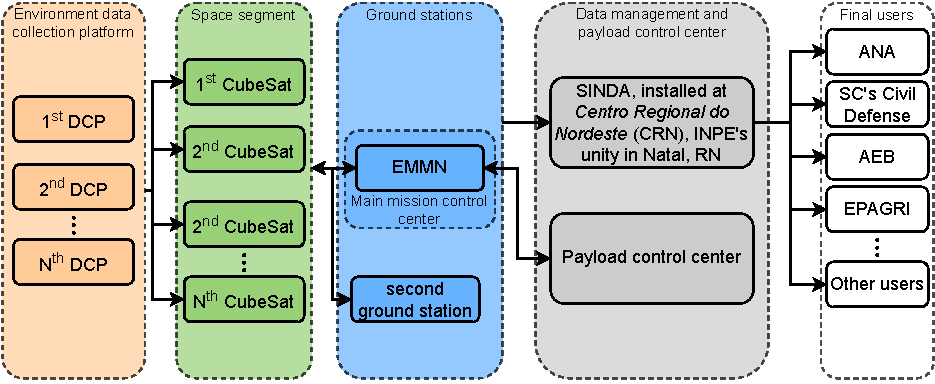
\includegraphics[width=0.9\columnwidth]{figures/mission_architecture.pdf}
        \caption{Catarina Constellation's mission architecture.}
        \label{fig:mission_architecture}
    \end{center}
\end{figure}

Catarina Constellation's mission architecture, presented in \autoref{fig:mission_architecture}, is designed to achieve the objectives set for the mission as a whole. We will therefore discuss how the Catarina-A1 fits into this architecture, presenting its particularities.

\subsection{Space Segment}

The Space Segment, as depicted in \autoref{fig:mission_architecture}, consists of multiple CubeSats, each of them with a service module and its payloads. It is noteworthy to mention that the Space Segment is designed with scalability in mind, allowing for future expansion by integrating additional CubeSats into the constellation. This expandability enhances the mission's resilience and facilitates maintenance, ensuring the sustainability of the Space Segment over time.

For the Catarina-A1, the service module is based on the reliable and proven FloripaSat-1, which provides the necessary infrastructure to host and operate the payloads efficiently. This platform encompasses essential subsystems such as \ac{EPS}, \ac{TTC}, and \ac{OBDH}.

The satellite carries two payloads, contributing to its functionality and mission objectives. The main payload is the \ac{EDC}, which is capable of receiving data from \acp{DCP} and the second one is the ExpLoRa, which utilizes LoRa technology to communicate with a specific SpaceLab's application.

% \subsection{Satellite platform}

% The main satellite's platform is based on the FloripaSat-1, which has a proven track record of reliability and performance. It provides the necessary environment to host and operate the payloads, as well as the essential systems of the satellite, such as ACS, \ac{EPS}, \ac{TTC}, and \ac{OBDH}.

% \subsection{Payloads}

% The satellite carries two payloads, one capable of receiving data from \acp{DCP}, and another that uses LoRa to communicate with a specific SpaceLab's application.

\subsection{Ground Segment}

As presented in \autoref{fig:mission_architecture}, the Ground Segment consists of \textit{(i)} \acp{DCP}, \textit{(ii)} the ground stations and \textit{(iii)} \ac{SINDA}, installed at \textit{Centro Regional do Nordeste} (\ac{INPE}'s unity).

Currently, \ac{SBCD} encompasses more than 1,000 stations, and due to its inherent scalability, it could expand to cover more areas in Brazil or even in other parts of South America, particularly remote ones. Regarding Catarina-A1, the satellite will collect data from a specific \ac{DCP}, located at Santa Catarina.

% Currently, \ac{SBCD} encompasses more than 1000 stations, and it is quite possible that it will grow in the future. Given its inherent scalability, it is thought that over time it will be extended to cover other regions of Brazil, particularly remote ones.

It is expected that there will be at least one ground station for the Catarina Constellation, which will be the mission's control center, the \ac{EMMN}. However, other ground stations could be used as ``secondary'' ones. In Catarina-A1's case, the \ac{EMMN} will be the main one, and a second ground station is planned, which will probably be installed at SpaceLab's facilities.

%The Catarina Constellation  ground stations include the main mission control center, the \ac{EMMN}, and possibly a secondary one, which could be established at the SpaceLab's facilities.

It is therefore generally expected that the \acp{DCP} will transmit data, which will be received by the satellite's \ac{EDC}. This would then be relayed to the \ac{EMMN} and then directed to \ac{SINDA} for processing and distribution to users.

\subsection{Mission control}

The \ac{EMMN}'s \ac{TTC} ground stations are responsible for tracking and controlling the satellite. In the baseline design, the \ac{EMMN} is used as the main tracking station. \ac{EMMN} was designed to operate in the \ac{VHF}, \ac{UHF} and S-Band, receiving payload-generated data and telemetry, as well as transmitting telecommands for satellites operating in low orbits.

The station performs autonomous tracking of several satellites according to a previous schedule and a scale of priorities. A ClientServer network design allows users to input and receive data remotely. Technical characteristics of the station can be found in \cite{emmn}.

% The mission control will be carried out by the Federal University of Santa Catarina (UFSC), which will monitor the health and performance of the satellite, execute flight control commands, and plan mission activities.

%\subsection{Communication protocols}

%\textcolor{red}{TODO}

% The mission uses a reliable communication protocol to ensure the transmission of data between the satellite and the ground segment. The protocol ensures that all transmitted data is received correctly and in order, and allows for error correction in transmission.

% Together, the mission architecture ensures that all functions and objectives of the mission can be fulfilled efficiently and effectively.

\section{Mission operation modes}

To enhance the comprehension of the satellite's operational modes, refer to the diagram in \autoref{fig:modes_diagram}. The depicted modes include: \ac{DM}, \ac{IM}, \ac{NM}, \ac{SBM}, and \ac{CM}.

\begin{figure}[H]
    \begin{center}
        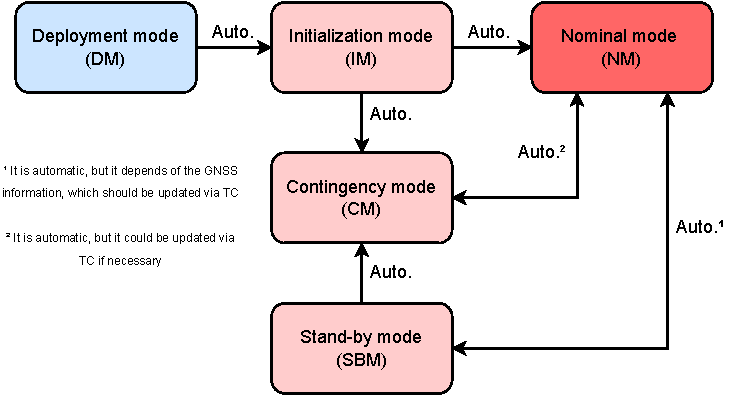
\includegraphics[width=0.8\textwidth]{figures/modes_diagram.pdf}
        \caption{Diagram of the satellite's operation modes.}
        \label{fig:modes_diagram}
    \end{center}
\end{figure}

Each mode will be delineated below, elucidating the specific occurrences during each phase and the transition mechanisms between them.

\subsection{\acl{DM} (DM)}

Throughout the launch phase, the satellite operates in \ac{DM}, during which all functions are temporarily deactivated to safeguard it amid the turbulent conditions. Following a successful launch and separation from the launch vehicle, the satellite is energized, seamlessly transitioning to the subsequent operating mode, the \ac{IM}.

\subsection{Initialization mode (IM)}

In \ac{IM}, the satellite undergoes an automatic power up, initiating the system initialization process. This sequence commences with the \ac{OBDH} subsystem, which systematically attempts to initialize the remaining subsystems in a specific order to assess their status and functionality.

During this phase, the antenna remains closed, a process anticipated to last 45 minutes. Upon completion of this period, the antennas will be deployed, and efforts are made to \textit{(i)} periodically transmit a beacon, and \textit{(ii)} determine the satellite's initial orientation (attitude). Once a communication link is established with the ground station, the satellite can transition to \ac{NM}, \ac{CM} or \ac{SBM}, depending on its orientation and status at the time.

\subsection{Nominal mode (NM)}

\begin{figure}[!ht]
    \begin{center}
        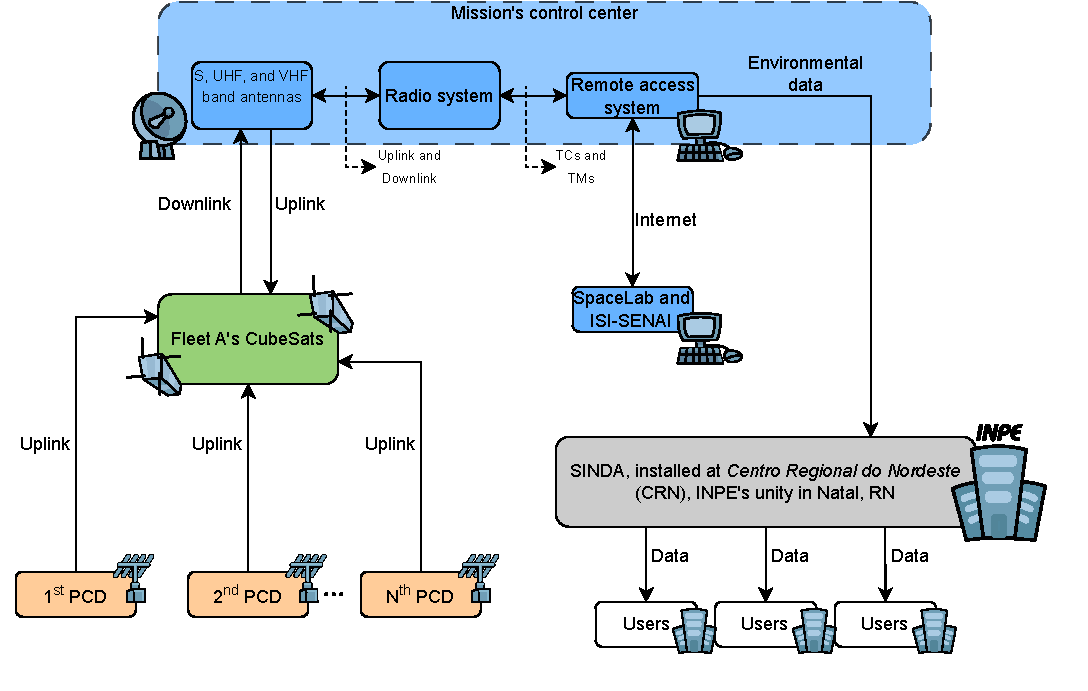
\includegraphics[width=\columnwidth]{figures/nm_operation.pdf}
        \caption{Description of the \ac{NM}' operations.}
        \label{fig:nm_operation}
    \end{center}
\end{figure}

This mode represents a power-negative state where the entire satellite is active. In this operational phase, both \ac{EDC} and ExpLoRa are functional – \ac{EDC} receives data from \acp{DCP}, while ExpLoRa receives information from a SpaceLab application. The activation and deactivation of this mode are controlled by GNSS information, ensuring that the satellite remains in \ac{NM} while within national territory.

Regarding the primary mission objective, illustrated in \autoref{fig:nm_operation}, the satellite receives data from \acp{DCP} and transmits it to the main mission's control center. In this center, the SpaceLab and \ac{ISI-SE} teams can remotely access the system for telecommand transmissions, and analysis/filtering of the received data.

\subsubsection{EDC and ExpLoRa activation}

The \ac{EDC} is essential for receiving data from the \ac{DCP} stations, which is the main objective of this mission. However, in order to optimize energy use and maximize operational efficiency, the \ac{EDC} will only be activated when the satellite is passing over Brazilian territory. This will allow the \ac{EDC} to collect data from the \acp{DCP} more efficiently and transmit it to the Ground Segment, conserving energy when data collection is not possible.

The decision of when to activate and deactivate the \ac{EDC} will be based on the satellite's orbit propagation, which will be calculated using regularly updated \acp{TLE}. \acp{TLE} are widely used format for describing a satellite's orbit. It consists of two lines of textual data that contain information about the orbital element epoch, inclination, right ascension of the ascending node, eccentricity, argument of perigee, mean anomaly, and mean motion of the satellite.

The satellite's \acp{TLE} will be received periodically from the Ground Segment. The mission control team will calculate the satellite's future position based on the \acp{TLE} and determine the period when the satellite will be over Brazil. During this period, the \ac{EDC} will be activated and begin collecting data from the \acp{DCP}. Once the satellite exits the coverage area, the \ac{EDC} will be deactivated until the next pass over Brazil.

The idea is to activate the ExpLoRa considering the same rule: only when the satellite is passing over Brazilian territory..

This approach of operating the \ac{EDC} and ExpLoRa based on orbit propagation allows for efficient utilization of satellite resources while maximizing the amount of data collected and transmitted to the Ground Segment.

\subsubsection{EDC and ExpLoRa deactivation}

Once the satellite moves beyond national territory, both payloads are deactivated to conserve energy. Consequently, the satellite transitions into the \ac{SBM}, with only the service module (comprising the \ac{OBDH}, \ac{EPS}, and \ac{TTC}) remaining powered.

\subsection{Stand-By mode (SBM)}

The \ac{OBDH} will then begin monitoring voltage and current levels, battery temperature, and other vital data gathered by the \ac{EPS} to assess the satellite's health. Periodically, the \ac{EPS} will transmit this information to the \ac{TTC} for redundancy. This setup enables potential issues to be diagnosed later when the satellite transmits telemetry back to Earth.

\subsection{Contingency mode (CM)}

The \ac{CM} is an operational state that the satellite enters if there is a failure in one of the critical systems or if an anomaly is detected. This includes the failure of one of the payloads or even other service module-related subsystem.

\subsubsection{Recovery procedure}

In the event of a failure \textit{(i)} the satellite may automatically attempt to reset one or more subsystems to analyze whether the problem has been solved or \textit{(ii)} the mission control team at \ac{UFSC} will send specific remote commands to make the satellite restart specific modules or completely disable some payload.

\section{Ground segment}

The Ground Segment is an essential component of the mission and includes all the terrestrial infrastructure that will be used to communicate with the satellite, receive data from the \ac{EDC} payload, and monitor the health and performance of the satellite.

\subsection{\aclp{DCP}}

The \acp{DCP} are ground stations distributed throughout Brazil that specialize in collecting environmental and other scientific data. In the case of Catarina-A1, the focus will be on the \acp{DCP} located in Florianópolis, SC, which will be the object of this mission.

This \ac{DCP} is initially defined as a platform provided by the Civil Defense of Santa Catarina. The most common model is a geotechnical \ac{DCP}, which captures soil humidity and pluviometric data and relays it to interested users. More technical details and the possibility of using different sensors for monitoring more parameters are yet \ac{TBD}.

The \ac{EDC} on board the satellite is designed to receive these data transmitted by the \acp{DCP}. When the satellite passes over the \ac{DCP} and the \ac{EDC} is activated, it will receive the data and store them for later transmission to the Ground Segment.

For ExpLoRa, a similar procedure will be carried out, but instead of a \ac{DCP}, an SpaceLab's \ac{IoT} application will send data to it.

\subsection{National System of Environmental Data}

The \ac{SINDA} is the main data reception center of \ac{INPE}. It is responsible for receiving the data transmitted by the satellite, processing it, and distributing it to end users. %\ac{SINDA} also plays an important role in monitoring the health and performance of the satellite.

% When the satellite is passing over SINDA and the communication link is established, the data collected by the \ac{EDC} will be transmitted to SINDA. Upon receipt, SINDA will process this data and make it available to end users.

% Additionally, SINDA will regularly receive telemetry from the satellite, allowing the mission control team to monitor the health and performance of the satellite and make operational decisions based on this information.

\subsection{Control and coordination}

The coordination and control of the Ground Segment will be carried out by the mission control team, which is responsible for ensuring that all parts of the Ground Segment are functioning correctly and for resolving any issues that may arise. They will also be responsible for determining when and where the \ac{EDC} should be activated based on the \acp{TLE} and the orbit propagation of the satellite.

In summary, the Ground Segment is a vital part of the mission. It enables data collection and transmission, satellite monitoring and control, and facilitates the interaction between the satellite and the \acp{DCP}, ensuring the success of the mission.

\section{Mission control}

Mission control will be carried out by \ac{UFSC}. \ac{UFSC} has a past involvement in satellite development, providing a wide range of skills and expertise to manage the satellite operation.

\subsection{Mission control station}

The main mission's control center is going to be the \ac{EMMN}, but \ac{UFSC} would like to establish a dedicated ground station this purpose, too. These stations will be responsible for the continuous monitoring of the satellite's health and performance.

\subsection{Mission control team}

The mission control team will be composed of students and professors from \ac{UFSC} who have been trained to operate the satellite system. The team will be responsible for monitoring the satellite's telemetry, identifying and resolving issues, and interfacing with other stakeholders, such as the teams responsible for the Ground Segment.

\subsection{Mission planning}

The \ac{UFSC} mission control team will also be responsible for planning and executing mission activities. This includes preparing detailed mission plans that define the activities to be performed by the satellite, such as activating the \ac{EDC} and collecting data from the \acp{DCP}. These mission plans will be based on the propagation of the satellite's orbit, which is calculated using the \acp{TLE}.

\subsection{Coordination with external entities}

As part of mission control, \ac{UFSC} will also coordinate with other entities involved in the mission, such as \ac{INPE} and the ground stations for data reception. This includes coordinating the upload of \acp{TLE} and the transmission of received data to \ac{INPE}'s \ac{SINDA} for processing and distribution.

In summary, \ac{UFSC} will have a central role in mission control, ensuring that the satellite operates efficiently and performs its tasks as planned. \ac{UFSC}'s extensive experience in mission operations will be a significant advantage for the success of this mission.

\section{Operational phase schedule}

\begin{table}[!htb]
    \centering
    \begin{tabular}{L{3cm}llL{7cm}}
        \toprule[1.5pt]
        \textbf{Experiment} & \textbf{Start} & \textbf{End} & \textbf{Observations} \\
        \midrule
        \acp{DCP} data reception          & Day 2 & End of lifespan & Continuous operation, subject to the availability of the \acp{DCP}. \\
        Data transmission            & Day 2 & End of lifespan & Data transmission will be performed as data is received from the \acp{DCP}. \\
        \bottomrule[1.5pt]
    \end{tabular}
    \caption{Steps of operation.}
    \label{tab:conops-schedule}
\end{table}
